%%%%% Elektrisches Feld %%%%%
%% #4 Elektronenbewegung im Elektrischen Feld %%


%Some sample text to be displayed above the first subsection

%\subsection{Prinzip}

%Ein Zyklotron besteht aus Zwei hohlen, halbzylindrischen und Duanden an denen eine Spannung mit unterschiedlichem Vorzeichen anliegt, und darüber bzw. darunter liegende Magneten, die ein homogenes Magnetfeld erzeugen. Zudem gibt es einen Einlass und einen Auslass für Teilchen.

%\begin{wrapfigure}{r}{0.4\textwidth} \label{Zyklo}
%
%	\vspace{-10pt}
%	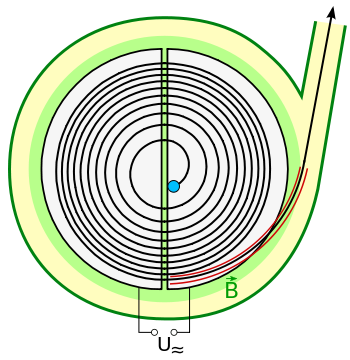
\includegraphics[width=0.35\textwidth]{Zyklotron_Prinzipskizze02.png}
%	\vspace{-13pt}
%	\caption{Prinzipskizze eines Zyklotrons}
%	\vspace{-5pt}	
%	
%\end{wrapfigure}

%\subsubsection{Anwendung}

% Some Formula:

%\begin{equation}
%	x= \frac{y \cdot 13 \pi z}
%			{\cos \alpha}
%\end{equation}

%%%%%%%%%%%%%%%%%%%%%%%
% Eigentlicher Beginn %
%%%%%%%%%%%%%%%%%%%%%%%


\begin{Wichtig}
Diese Bewegungsgesetze und Bewegungsgesetze allgemein sind wiederkehrendes Grundmaterial in der Schulphysik und sollten daher \glqq aus dem FF\grqq{} beherrscht werden.
\end{Wichtig}

\subsection{Bewegung parallel zu den Feldlinien} \label{subsec:BewegungsgesetzParallel}

Auf ruhende Elektronen, oder Elektronen, die sich parallel zu den Feldlinien des elektrischen Feldes bewegen, wirkt ein Kraft, welche sie ebenfalls parallel zu den Feldlinien beschleunigt. Daher ist und bleibt diese Bewegung eindimensional und sie lässt sich durch \emph{ein} Weg-Zeit Gesetz der gleichmäßig beschleunigten Bewegung ausdrücken:

%%%%%%%%%%%%%%%%%%%%%
% WEG ZEIT GESETZE %%
%%%%%%%%%%%%%%%%%%%%%

Nach Newton gilt $F = m \cdot a$, was sich zu $a = \frac{F}{m}$ umstellen lässt. $F_{el}$ (Siehe: \gleichungsreferenz{eq:F_el}) lässt sich nun für $F$ einsetzten und die Elektronenmasse $m_e$, welche konstant ist (\casio{03}), für $m$:

\begin{equation}
	a = \frac{q_e \cdot E}{m_e}
\end{equation}


Folgendes Weg-Zeit-Gesetz für den Weg der Feldlinien entgegen, lässt sich aufstellen:

\begin{align} \label{eq:s(t)Allgemein}
\begin{split}
	s(t) &= \frac{1}{2} a \cdot t^2 + v_0 \cdot t + s_0 \\
	s(t) &= \frac{q_e \cdot E}{2m_e} \cdot t^2 + v_0 \cdot t + s_0
\end{split}
\end{align}

\noindent In diesem Fall steht $v_0$ für die angesprochene mögliche Anfangsgeschwindigkeit, die das Elektron bereits \glqq drauf hatte\grqq{} und $s_0$ für eine mögliche Anfangsstrecke, die das Elektron vor Beeinflussung durch das elektrische Feld schon zurückgelegt hatte.

\begin{Wichtig}
Beim Einsetzen von $v_0$ auf das Vorzeichen achten! Z.B. muss eine Geschwindigkeit, die der Beschleunigungsrichtung  entgegengesetzt ist, also in Richtung der Feldlinien verläuft, mit negativem Vorzeichen notiert werden.
\end{Wichtig}

Dieses Gesetz kann spezifischer für die Bewegung in einem Plattenkondensator mit eingesetztem $E=\frac{U}{d}$ (Siehe \gleichungsreferenz{eq:feldstaerke_kondensator}) ausgedrückt werden:

\begin{align} \label{eq:s(t)imKondensator}
\begin{split}
	s(t) = \frac{q_e \cdot U}{2d \cdot m_e} \cdot t^2 + v_0 \cdot t + s_0
\end{split}
\end{align}


\subsection{Bewegung senkrecht zu den Feldlinien} \label{subsec:BewegungsgesetzSenkrecht}

Etwas komplexer wird es, wenn sich ein Elektron bereits senkrecht zu den Feldlinien eines elektrischen Feldes bewegt. Analog zu den Berechnungen eines horizontalen Wurfs (z.B. Abwurf von Ladung von einem Flugzeug) muss auch hier die Bewegung in eine horizontale Bewegung (\glqq in x-Richtung\grqq) und eine vertikale Bewegung (\glqq in y-Richtung\grqq) aufgeteilt werden. 

Die Bewegung in x-Richtung ist als einfache gleichförmige Bewegung nach $x(t)=v \cdot t + x_0$ zu beschreiben. 

Die Bewegung in y-Richtung kann aus Gleichung \ref{eq:s(t)Allgemein} oder \ref{eq:s(t)imKondensator} übernommen werden.

Um beide Bewegungen in einer einzigen Gleichung zusammenzufassen, also den y-Weg in Abhängigkeit der x-Position anzugeben und damit die Position des Elektrons eindeutig zu bestimmen, muss $x(t)$ nach $t$ umgestellt werden und dieses $t$ in die Gleichung von $s(t)$ eingesetzt werden. 

\begin{NiceToKnow}
Zur Vereinfachung wird in den aller-allermeisten Aufgaben zu diesem Thema aus einen Anfangswert, also auf $v_0$, $y_0$ o.ä. verzichtet. So auch in dieser Herleitung.
\end{NiceToKnow}

Zudem wird die Funktion für den Weg in y-Richtung nicht mehr $s(t)$, sondern $y(t)$ genannt, um sie besser von $x(t)$ abzugrenzen.

\begin{align} \label{eq:x(t)Senkrecht}
\begin{split}
	x(t) &= v_x \cdot t \\
	t(x) &= \frac{x}{v}
\end{split}
\end{align}

\noindent Es folgt das Einsetzten in die allgemeine Form von $y(t)$ (Siehe: \gleichungsreferenz{eq:s(t)Allgemein}):

\begin{align} \label{eq:y(x)Allgemein}
\begin{split}
	y(t) &= \frac{q_e \cdot E}{2m_e} \cdot t^2 \\
	y(x) &= \frac{q_e \cdot E}{2m_e} \cdot \frac{x^2}{v_{x}^2}
\end{split}
\end{align}

\noindent Spezifisch für einen Kondensator:

\begin{align} \label{eq:y(x)imKondensator}
\begin{split}
	y(t) &= \frac{q_e \cdot U}{2d \cdot m_e} \cdot t^2 \\
	y(x) &= \frac{q_e \cdot U}{2d \cdot m_e} \cdot \frac{x^2}{v_{x}^2}
\end{split}
\end{align}





